\chapter{Refractive Index}

\section{Aim}
To learn how to determine the refractive index of a glass block

\section{Background Information}
A straight pen appears bent when it is partially immersed in a glass of water. This is due to the light rays bending when they leave the water. The bending of light when it passes from one medium to another different medium is known as refraction. The refractive index is a constant of a material that determines how much the light will bend when it enters that medium from a vacuum. Manufacturers in industries need to know how to calculate the index of refraction of a material for proper construction of optical instruments such as glasses, telescopes, binoculars, etc. How do we calculate it?

\section{Materials}
Glass block, 4 optical pins, 4 drawing pins, protractor, plain paper, ruler, soft board, and a pencil

\section{Procedure}
\begin{enumerate}
\item Fix a white sheet of paper on a soft board by using drawing pins.
\item Place the glass block flat on the sheet of paper and trace along the outside using a pencil.
\item Remove the block and label the corners ABCD (see figure).
\item Using a protractor, draw a line NM perpendicular to AB, which is near corner A.
\item Draw another line RQ which makes an angle of incidence, $i_1$, equal to $20^\circ$ with line NM.
\item Replace the block back on the sheet of paper inside the box ABCD. Insert optical pins at two different points along the line RQ. 
\item Observe these optical pins through the glass block from the opposite side CD. Place two more optical pins on this side of the block so that they appear to be in line with the original two pins on the other side. 
\item Remove the block and pins. Draw a line through the points of the two new optical pins until the line touches the outline of the glass block and label the intersection P$_1$.
\item Draw a line which connects Q and P$_1$. Measure and record the angle of refraction, $r_1$.
\item Repeat steps 5 - 9 for angles of incidence $i_2-i_5$ equal to $30^\circ$, $40^\circ$, $50^\circ$ and $60^\circ$. 
\item Tabulate your results.
\end{enumerate}


\begin{figure}[h!]
\centering
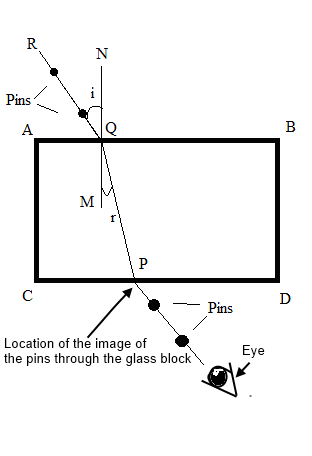
\includegraphics[width=8cm]{./img/refractive-index-1.png}
\caption{Refractive Index practical setup}
\label{fig:refractive-index-1}
\end{figure}

\section{Analysis and Interpretation}
\begin{enumerate}
\item Calculate $\sin(i)$ and $\sin(r)$ for each incident angle $i$ and angle of refraction $r$.  
\item Calculate $\cfrac{\sin(i)}{\sin(r)}$ for each incident angle and angle of refraction. 
\item Plot a graph of $\sin(i)$ against $\sin(r)$.
\item Determine the slope of the graph. What does it represent?
\end{enumerate}

\section{Conclusion}
What is the index of refraction of the glass block?

\section{Questions for Discussion}
\begin{enumerate}
\item What happened to the angle of refraction as the angle of incidence increased?
\item What would happen to the angle of refraction when the angle of incidence is (i) $0^\circ$ and (ii) $90^\circ$?
\end{enumerate}

\section{Reflection and Self Assessment}
\begin{enumerate}
\item How can the knowledge of this experiment be used in your daily life? 
\item How does this experiment relate to the illusion of seeing a pond on the road during a hot and sunny day?
\end{enumerate}